\newpage 
\section{Spanning trees}

\begin{Def}[Spanning Tree]

    A \textbf{spanning tree} of a graph $G$ is a subgraph containing edges to each $n\in G$ without cycles.
\end{Def}

\begin{Def}[Minimum Spanning Tree (MST)]

    A \textbf{minimum spanning tree} of a graph $G$ is a spanning tree with the smallest sum of edge weights.
\end{Def}

\begin{figure}[h]
    \centering
    



    \tikzset{every picture/.style={line width=0.75pt}} %set default line width to 0.75pt        

    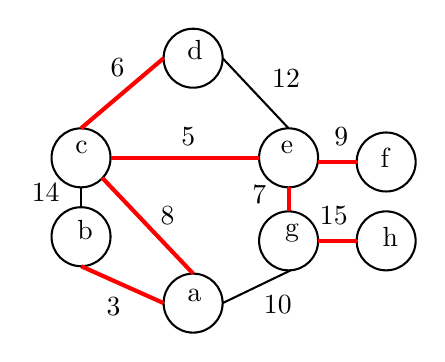
\begin{tikzpicture}[x=0.75pt,y=0.75pt,yscale=-1,xscale=1]
    %uncomment if require: \path (0,300); %set diagram left start at 0, and has height of 300
    
    %Shape: Circle [id:dp2026334324662925] 
    \draw  [fill={rgb, 255:red, 255; green, 255; blue, 255 }  ,fill opacity=1 ] (173.33,153.21) .. controls (173.33,145.36) and (179.69,139) .. (187.54,139) .. controls (195.39,139) and (201.75,145.36) .. (201.75,153.21) .. controls (201.75,161.06) and (195.39,167.42) .. (187.54,167.42) .. controls (179.69,167.42) and (173.33,161.06) .. (173.33,153.21) -- cycle ;
    %Shape: Circle [id:dp026171578812805518] 
    \draw  [fill={rgb, 255:red, 255; green, 255; blue, 255 }  ,fill opacity=1 ] (173.33,115.21) .. controls (173.33,107.36) and (179.69,101) .. (187.54,101) .. controls (195.39,101) and (201.75,107.36) .. (201.75,115.21) .. controls (201.75,123.06) and (195.39,129.42) .. (187.54,129.42) .. controls (179.69,129.42) and (173.33,123.06) .. (173.33,115.21) -- cycle ;
    %Shape: Circle [id:dp2560123313690592] 
    \draw  [fill={rgb, 255:red, 255; green, 255; blue, 255 }  ,fill opacity=1 ] (227.33,185.21) .. controls (227.33,177.36) and (233.69,171) .. (241.54,171) .. controls (249.39,171) and (255.75,177.36) .. (255.75,185.21) .. controls (255.75,193.06) and (249.39,199.42) .. (241.54,199.42) .. controls (233.69,199.42) and (227.33,193.06) .. (227.33,185.21) -- cycle ;
    %Shape: Circle [id:dp08670120448085128] 
    \draw  [fill={rgb, 255:red, 255; green, 255; blue, 255 }  ,fill opacity=1 ] (227.33,67.21) .. controls (227.33,59.36) and (233.69,53) .. (241.54,53) .. controls (249.39,53) and (255.75,59.36) .. (255.75,67.21) .. controls (255.75,75.06) and (249.39,81.42) .. (241.54,81.42) .. controls (233.69,81.42) and (227.33,75.06) .. (227.33,67.21) -- cycle ;
    %Shape: Circle [id:dp6890620040174518] 
    \draw  [fill={rgb, 255:red, 255; green, 255; blue, 255 }  ,fill opacity=1 ] (273.33,115.21) .. controls (273.33,107.36) and (279.69,101) .. (287.54,101) .. controls (295.39,101) and (301.75,107.36) .. (301.75,115.21) .. controls (301.75,123.06) and (295.39,129.42) .. (287.54,129.42) .. controls (279.69,129.42) and (273.33,123.06) .. (273.33,115.21) -- cycle ;
    %Shape: Circle [id:dp062427767698108316] 
    \draw  [fill={rgb, 255:red, 255; green, 255; blue, 255 }  ,fill opacity=1 ] (273.33,155.21) .. controls (273.33,147.36) and (279.69,141) .. (287.54,141) .. controls (295.39,141) and (301.75,147.36) .. (301.75,155.21) .. controls (301.75,163.06) and (295.39,169.42) .. (287.54,169.42) .. controls (279.69,169.42) and (273.33,163.06) .. (273.33,155.21) -- cycle ;
    %Shape: Circle [id:dp4615260186128455] 
    \draw   (320.33,155.21) .. controls (320.33,147.36) and (326.69,141) .. (334.54,141) .. controls (342.39,141) and (348.75,147.36) .. (348.75,155.21) .. controls (348.75,163.06) and (342.39,169.42) .. (334.54,169.42) .. controls (326.69,169.42) and (320.33,163.06) .. (320.33,155.21) -- cycle ;
    %Shape: Circle [id:dp46014483622543756] 
    \draw  [fill={rgb, 255:red, 255; green, 255; blue, 255 }  ,fill opacity=1 ] (320.33,117.21) .. controls (320.33,109.36) and (326.69,103) .. (334.54,103) .. controls (342.39,103) and (348.75,109.36) .. (348.75,117.21) .. controls (348.75,125.06) and (342.39,131.42) .. (334.54,131.42) .. controls (326.69,131.42) and (320.33,125.06) .. (320.33,117.21) -- cycle ;
    %Straight Lines [id:da8329795884294181] 
    \draw    (187.54,139) -- (187.54,129.42) ;
    %Straight Lines [id:da27990445195837865] 
    \draw [color={rgb, 255:red, 255; green, 0; blue, 0 }  ,draw opacity=1 ][line width=1.5]    (227.33,67.21) -- (187.54,101) ;
    %Straight Lines [id:da6849646426209853] 
    \draw [color={rgb, 255:red, 255; green, 0; blue, 0 }  ,draw opacity=1 ][line width=1.5]    (227.33,185.21) -- (187.54,167.42) ;
    %Straight Lines [id:da17487697052764262] 
    \draw [color={rgb, 255:red, 255; green, 0; blue, 0 }  ,draw opacity=1 ][line width=1.5]    (201.75,115.21) -- (273.33,115.21) ;
    %Straight Lines [id:da6321202969865173] 
    \draw [color={rgb, 255:red, 255; green, 0; blue, 0 }  ,draw opacity=1 ][line width=1.5]    (197.75,124.82) -- (241.54,171) ;
    %Straight Lines [id:da8393601584465114] 
    \draw    (255.75,185.21) -- (288.54,169.42) ;
    %Straight Lines [id:da8447960149171586] 
    \draw [color={rgb, 255:red, 255; green, 0; blue, 0 }  ,draw opacity=1 ][line width=1.5]    (287.54,141) -- (287.54,129.42) ;
    %Straight Lines [id:da3450940906788029] 
    \draw [color={rgb, 255:red, 255; green, 0; blue, 0 }  ,draw opacity=1 ][line width=1.5]    (320.33,155.21) -- (301.75,155.21) ;
    %Straight Lines [id:da8922618638234496] 
    \draw [color={rgb, 255:red, 255; green, 0; blue, 0 }  ,draw opacity=1 ][line width=1.5]    (320.33,117.21) -- (301.75,117.21) ;
    %Straight Lines [id:da7285203318813096] 
    \draw    (287.54,101) -- (255.75,67.21) ;
    
    % Text Node
    \draw (200.33,66) node [anchor=north west][inner sep=0.75pt]   [align=left] {6};
    % Text Node
    \draw (234.33,99) node [anchor=north west][inner sep=0.75pt]   [align=left] {5};
    % Text Node
    \draw (224.33,137) node [anchor=north west][inner sep=0.75pt]   [align=left] {8};
    % Text Node
    \draw (162.33,126) node [anchor=north west][inner sep=0.75pt]   [align=left] {14};
    % Text Node
    \draw (198.33,181) node [anchor=north west][inner sep=0.75pt]   [align=left] {3};
    % Text Node
    \draw (274.15,180.31) node [anchor=north west][inner sep=0.75pt]   [align=left] {10};
    % Text Node
    \draw (301.15,137.31) node [anchor=north west][inner sep=0.75pt]   [align=left] {15};
    % Text Node
    \draw (308.15,99.31) node [anchor=north west][inner sep=0.75pt]   [align=left] {9};
    % Text Node
    \draw (278.15,71.31) node [anchor=north west][inner sep=0.75pt]   [align=left] {12};
    % Text Node
    \draw (237.33,177) node [anchor=north west][inner sep=0.75pt]   [align=left] {a};
    % Text Node
    \draw (184.33,144) node [anchor=north west][inner sep=0.75pt]   [align=left] {b};
    % Text Node
    \draw (183.33,106) node [anchor=north west][inner sep=0.75pt]   [align=left] {c};
    % Text Node
    \draw (237.33,57) node [anchor=north west][inner sep=0.75pt]   [align=left] {d};
    % Text Node
    \draw (282.33,106) node [anchor=north west][inner sep=0.75pt]   [align=left] {e};
    % Text Node
    \draw (330.33,109) node [anchor=north west][inner sep=0.75pt]   [align=left] {f};
    % Text Node
    \draw (284.33,146) node [anchor=north west][inner sep=0.75pt]   [align=left] {g};
    % Text Node
    \draw (331.33,147) node [anchor=north west][inner sep=0.75pt]   [align=left] {h};
    % Text Node
    \draw (268.6,127) node [anchor=north west][inner sep=0.75pt]   [align=left] {7};
    
    
    \end{tikzpicture}

    \caption{Example of an graph with MST highlighted in red.}
    \label{fig:mst_example}

\end{figure}
\noindent
This tree visits each node once taking the shortest path which connects all of them.

\noindent
\textbf{Possible Algorithms:}
\begin{itemize}
    \item \textbf{Prim's:} Start with some root node s. Grow a tree T from s outward. At each step, add to T the cheapest edge e with exactly one endpoint in T.
    \item \textbf{Kruskal's:} Start with \( T = \emptyset \). Consider edges in ascending order of weights. Insert edge e in T unless doing so would create a cycle.
    \item \textbf{Reverse-Delete:} Start with \( T = E \). Consider edges in descending order of weights. Delete edge e from T unless doing so would disconnect T.
    \item \textbf{Borůvka's:} Start with \( T = \emptyset \). At each round, add the cheapest edge leaving each connected component of T. Terminates after at most \( \log(n) \) rounds.
\end{itemize}

\noindent
Next we revisit cycles and introduce \textbf{cuts}, which will have important implications when approaching this problem.

\newpage

\begin{Def}[Endpoint]
    
        An \textbf{endpoint} is either end of an edge. So for edge $e = u\leftrightarrow v$, $u$ and $v$ are endpoints. If
        $u\to v$, then $v$ is an endpoint of $u$.
\end{Def}
\begin{Def}[Cut]

    Given a graph $G$, partitioning of the nodes into a set is called a \textbf{cut}, say $G'$. Nodes, with exactly one endpoint in $G'$, are the \textbf{cut-set}.
    
\end{Def}



\begin{figure}[h]
    \centering
    

\tikzset{every picture/.style={line width=0.75pt}} %set default line width to 0.75pt        

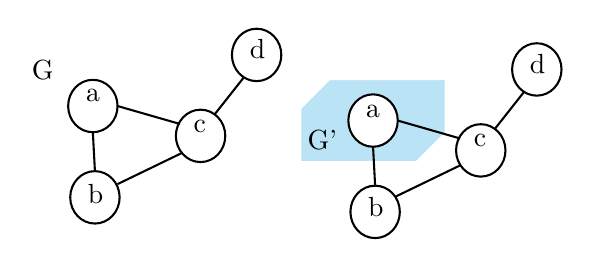
\begin{tikzpicture}[x=0.75pt,y=0.75pt,yscale=-1,xscale=1]
%uncomment if require: \path (0,265); %set diagram left start at 0, and has height of 265

%Snip Diagonal Corner Rect [id:dp03818061283377061] 
\draw  [color={rgb, 255:red, 255; green, 255; blue, 255 }  ,draw opacity=1 ][fill={rgb, 255:red, 96; green, 190; blue, 232 }  ,fill opacity=0.43 ] (263.9,142.63) -- (319.9,142.63) -- (319.9,142.63) -- (319.9,168.63) -- (305.9,182.63) -- (249.9,182.63) -- (249.9,182.63) -- (249.9,156.63) -- cycle ;
%Shape: Ellipse [id:dp6461843193531308] 
\draw   (138,155.63) .. controls (138,148.65) and (143.33,143) .. (149.9,143) .. controls (156.47,143) and (161.8,148.65) .. (161.8,155.63) .. controls (161.8,162.6) and (156.47,168.25) .. (149.9,168.25) .. controls (143.33,168.25) and (138,162.6) .. (138,155.63) -- cycle ;
%Shape: Ellipse [id:dp36167987939288815] 
\draw   (139,199.63) .. controls (139,192.65) and (144.33,187) .. (150.9,187) .. controls (157.47,187) and (162.8,192.65) .. (162.8,199.63) .. controls (162.8,206.6) and (157.47,212.25) .. (150.9,212.25) .. controls (144.33,212.25) and (139,206.6) .. (139,199.63) -- cycle ;
%Shape: Ellipse [id:dp21386485914880626] 
\draw   (189.9,170) .. controls (189.9,163.03) and (195.23,157.38) .. (201.8,157.38) .. controls (208.37,157.38) and (213.7,163.03) .. (213.7,170) .. controls (213.7,176.97) and (208.37,182.63) .. (201.8,182.63) .. controls (195.23,182.63) and (189.9,176.97) .. (189.9,170) -- cycle ;
%Straight Lines [id:da11599175466120859] 
\draw    (161.8,155.63) -- (191.8,164.25) ;
%Straight Lines [id:da8317457413146321] 
\draw    (149.9,168.25) -- (150.9,187) ;
%Shape: Ellipse [id:dp995295032837351] 
\draw  [fill={rgb, 255:red, 255; green, 255; blue, 255 }  ,fill opacity=1 ] (273,162.63) .. controls (273,155.65) and (278.33,150) .. (284.9,150) .. controls (291.47,150) and (296.8,155.65) .. (296.8,162.63) .. controls (296.8,169.6) and (291.47,175.25) .. (284.9,175.25) .. controls (278.33,175.25) and (273,169.6) .. (273,162.63) -- cycle ;
%Shape: Ellipse [id:dp8597498314367041] 
\draw   (274,206.63) .. controls (274,199.65) and (279.33,194) .. (285.9,194) .. controls (292.47,194) and (297.8,199.65) .. (297.8,206.63) .. controls (297.8,213.6) and (292.47,219.25) .. (285.9,219.25) .. controls (279.33,219.25) and (274,213.6) .. (274,206.63) -- cycle ;
%Shape: Ellipse [id:dp24205568125740362] 
\draw   (324.9,177) .. controls (324.9,170.03) and (330.23,164.38) .. (336.8,164.38) .. controls (343.37,164.38) and (348.7,170.03) .. (348.7,177) .. controls (348.7,183.97) and (343.37,189.63) .. (336.8,189.63) .. controls (330.23,189.63) and (324.9,183.97) .. (324.9,177) -- cycle ;
%Straight Lines [id:da5757559450680038] 
\draw    (296.8,162.63) -- (326.8,171.25) ;
%Straight Lines [id:da9921369924680631] 
\draw    (284.9,175.25) -- (285.9,194) ;
%Straight Lines [id:da696315279326696] 
\draw    (161.8,193.25) -- (192.8,178.25) ;
%Straight Lines [id:da9313904515500769] 
\draw    (295.8,199.25) -- (326.8,184.25) ;
%Shape: Ellipse [id:dp6136012462910496] 
\draw   (216.9,131) .. controls (216.9,124.03) and (222.23,118.38) .. (228.8,118.38) .. controls (235.37,118.38) and (240.7,124.03) .. (240.7,131) .. controls (240.7,137.97) and (235.37,143.63) .. (228.8,143.63) .. controls (222.23,143.63) and (216.9,137.97) .. (216.9,131) -- cycle ;
%Straight Lines [id:da5907253154079168] 
\draw    (222.8,141.63) -- (208.8,159.38) ;
%Shape: Ellipse [id:dp9497617675815347] 
\draw   (351.9,138) .. controls (351.9,131.03) and (357.23,125.38) .. (363.8,125.38) .. controls (370.37,125.38) and (375.7,131.03) .. (375.7,138) .. controls (375.7,144.97) and (370.37,150.63) .. (363.8,150.63) .. controls (357.23,150.63) and (351.9,144.97) .. (351.9,138) -- cycle ;
%Straight Lines [id:da7693110411499856] 
\draw    (357.8,148.63) -- (343.8,166.38) ;

% Text Node
\draw (145,146) node [anchor=north west][inner sep=0.75pt]   [align=left] {a};
% Text Node
\draw (146,192) node [anchor=north west][inner sep=0.75pt]   [align=left] {b};
% Text Node
\draw (197,161) node [anchor=north west][inner sep=0.75pt]   [align=left] {c};
% Text Node
\draw (280,154) node [anchor=north west][inner sep=0.75pt]   [align=left] {a};
% Text Node
\draw (332,168) node [anchor=north west][inner sep=0.75pt]   [align=left] {c};
% Text Node
\draw (281,198) node [anchor=north west][inner sep=0.75pt]   [align=left] {b};
% Text Node
\draw (119,132) node [anchor=north west][inner sep=0.75pt]   [align=left] {G};
% Text Node
\draw (251.9,165.63) node [anchor=north west][inner sep=0.75pt]   [align=left] {G'};
% Text Node
\draw (224,122) node [anchor=north west][inner sep=0.75pt]   [align=left] {d};
% Text Node
\draw (359,129) node [anchor=north west][inner sep=0.75pt]   [align=left] {d};


\end{tikzpicture}

    \caption{Illustration of a graph $G$ and a cut $G'$ of the graph.}
    \label{fig:cut_example}
\end{figure}
\noindent
We see in Figure (\ref{fig:cut_example}) that $G'=\{a\}$ and our cut-set contains edge-pairs $(a,b)$ and $(a,c)$. Where the edge $(d,c)$ is not included as the cut $G'$ does not intersect it.
\begin{theo}[Cycles \& Cut-sets]

    If a cut-set crosses a cycle, then the cut-set intersects an even number of edges in the cycle.\\
    As what comes in, must come out.
\end{theo}
\noindent
Given Figure (\ref{fig:cut_example}), the cut-set $G'$ intersects the cycle $(a,b,c)$, yielding an even cut-set.
\begin{theo}[Cycle Property]
    
    In a graph with a cycle, the edge with the largest weight in that cycle is not in the MST.
    As taking an edge from a cycle does not disconnect the graph, the largest edge is not necessary.
\end{theo}
\begin{theo}[Cut Property]

    Given a graph $G$ and a cut-set $C$, where $e$ is the lightest-edge in $C$; $e$ must be in the MST. As if $e\notin G$ and $G$ is an MST, adding $e$ creates a cycle. By the cycle property, $e$ must replace the heaviest edge in that cycle.
\end{theo}


\newpage
\noindent
\textbf{Example:} Given the below Figure (\ref{fig:cut_property}), point $e$ must be in the MST to connect all nodes (cut property). Say dash-edge $f$ is the largest in its cycle, then $f$ is not in the MST (cycle property).
\begin{figure}[h]
    \centering
    

\tikzset{every picture/.style={line width=0.75pt}} %set default line width to 0.75pt        

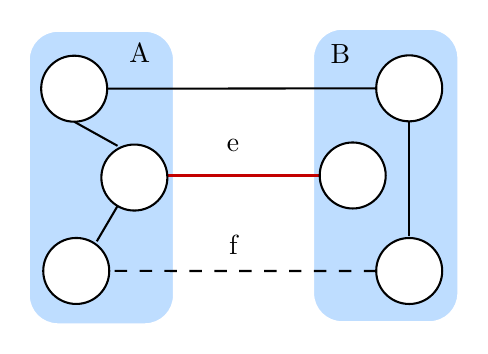
\begin{tikzpicture}[x=0.75pt,y=0.75pt,yscale=-1,xscale=1]
%uncomment if require: \path (0,300); %set diagram left start at 0, and has height of 300

%Rounded Rect [id:dp49102406805739185] 
\draw  [color={rgb, 255:red, 255; green, 255; blue, 255 }  ,draw opacity=1 ][fill={rgb, 255:red, 139; green, 194; blue, 255 }  ,fill opacity=0.56 ] (166,94) .. controls (166,86.27) and (172.27,80) .. (180,80) -- (222,80) .. controls (229.73,80) and (236,86.27) .. (236,94) -- (236,207.42) .. controls (236,215.15) and (229.73,221.42) .. (222,221.42) -- (180,221.42) .. controls (172.27,221.42) and (166,215.15) .. (166,207.42) -- cycle ;
%Rounded Rect [id:dp35224359948314676] 
\draw  [color={rgb, 255:red, 255; green, 255; blue, 255 }  ,draw opacity=1 ][fill={rgb, 255:red, 139; green, 194; blue, 255 }  ,fill opacity=0.56 ] (303,93) .. controls (303,85.27) and (309.27,79) .. (317,79) -- (359,79) .. controls (366.73,79) and (373,85.27) .. (373,93) -- (373,206.42) .. controls (373,214.15) and (366.73,220.42) .. (359,220.42) -- (317,220.42) .. controls (309.27,220.42) and (303,214.15) .. (303,206.42) -- cycle ;
%Straight Lines [id:da3016657209067013] 
\draw [color={rgb, 255:red, 195; green, 0; blue, 0 }  ,draw opacity=1 ]   (306.2,149.71) -- (232.8,149.71) ;
%Shape: Circle [id:dp005421762108458239] 
\draw  [fill={rgb, 255:red, 255; green, 255; blue, 255 }  ,fill opacity=1 ] (172,107.9) .. controls (172,99.12) and (179.12,92) .. (187.9,92) .. controls (196.68,92) and (203.8,99.12) .. (203.8,107.9) .. controls (203.8,116.68) and (196.68,123.8) .. (187.9,123.8) .. controls (179.12,123.8) and (172,116.68) .. (172,107.9) -- cycle ;
%Shape: Circle [id:dp4707156627783562] 
\draw  [fill={rgb, 255:red, 255; green, 255; blue, 255 }  ,fill opacity=1 ] (201,150.71) .. controls (201,141.93) and (208.12,134.81) .. (216.9,134.81) .. controls (225.68,134.81) and (232.8,141.93) .. (232.8,150.71) .. controls (232.8,159.49) and (225.68,166.61) .. (216.9,166.61) .. controls (208.12,166.61) and (201,159.49) .. (201,150.71) -- cycle ;
%Shape: Circle [id:dp7864251820189283] 
\draw  [fill={rgb, 255:red, 255; green, 255; blue, 255 }  ,fill opacity=1 ] (173,195.71) .. controls (173,186.93) and (180.12,179.81) .. (188.9,179.81) .. controls (197.68,179.81) and (204.8,186.93) .. (204.8,195.71) .. controls (204.8,204.49) and (197.68,211.61) .. (188.9,211.61) .. controls (180.12,211.61) and (173,204.49) .. (173,195.71) -- cycle ;
%Straight Lines [id:da6423097124480006] 
\draw    (208.8,164.43) -- (198.8,181.43) ;
%Straight Lines [id:da19288845816924016] 
\draw    (187.9,123.8) -- (208.8,135.43) ;
%Shape: Circle [id:dp4761241780620117] 
\draw  [fill={rgb, 255:red, 255; green, 255; blue, 255 }  ,fill opacity=1 ] (333.42,107.73) .. controls (333.42,98.95) and (340.54,91.83) .. (349.32,91.83) .. controls (358.1,91.83) and (365.22,98.95) .. (365.22,107.73) .. controls (365.22,116.51) and (358.1,123.63) .. (349.32,123.63) .. controls (340.54,123.63) and (333.42,116.51) .. (333.42,107.73) -- cycle ;
%Shape: Circle [id:dp6465860920913904] 
\draw  [fill={rgb, 255:red, 255; green, 255; blue, 255 }  ,fill opacity=1 ] (306.2,149.71) .. controls (306.2,140.93) and (313.32,133.81) .. (322.1,133.81) .. controls (330.88,133.81) and (338,140.93) .. (338,149.71) .. controls (338,158.49) and (330.88,165.61) .. (322.1,165.61) .. controls (313.32,165.61) and (306.2,158.49) .. (306.2,149.71) -- cycle ;
%Shape: Circle [id:dp2663185207581561] 
\draw  [fill={rgb, 255:red, 255; green, 255; blue, 255 }  ,fill opacity=1 ] (333.42,195.73) .. controls (333.42,186.95) and (340.54,179.83) .. (349.32,179.83) .. controls (358.1,179.83) and (365.22,186.95) .. (365.22,195.73) .. controls (365.22,204.51) and (358.1,211.63) .. (349.32,211.63) .. controls (340.54,211.63) and (333.42,204.51) .. (333.42,195.73) -- cycle ;
%Straight Lines [id:da6545330759865682] 
\draw  [dash pattern={on 4.5pt off 4.5pt}]  (333.42,195.73) -- (204.8,195.71) ;
%Straight Lines [id:da23327256965954069] 
\draw    (333.42,107.73) -- (203.8,107.9) ;
%Straight Lines [id:da6594941535881259] 
\draw    (349.32,123.63) -- (349.32,178.83) ;

% Text Node
\draw (260,131) node [anchor=north west][inner sep=0.75pt]   [align=left] {e};
% Text Node
\draw (213,84.48) node [anchor=north west][inner sep=0.75pt]   [align=left] {A};
% Text Node
\draw (310,85) node [anchor=north west][inner sep=0.75pt]   [align=left] {B};
% Text Node
\draw (261,177) node [anchor=north west][inner sep=0.75pt]   [align=left] {f};


\end{tikzpicture}
    
    \caption{A graph cut into two disjoint sets, with a highlighted edge $e$ and a dashed edge $f$.}
    \label{fig:cut_property}
\end{figure}

\vspace{-1em}
\begin{theo}[Prim's Algorithm]

    Given a connected graph $G$ with $n$ nodes and $m$ edges,
    \begin{enumerate}
        \item [(i.)] Initialize an MST table $T$, and a priority queue $Q$ with each $n$ of weight $\infty$.
        \item [(ii.)] Start a round with an arbitrary node $s$, adding children nodes $v$ to the queue.
        \item [(iii.)] Update each $T[v]=s$, if $w(s,v)$ is lighter than $T[v]$.
        \item [(iv.)] End this round, take the top node in $Q$ as the new $s$, repeat (ii.)-(iv.) until all $n\in T$.
    \end{enumerate}
    \noindent

\end{theo}

\vspace{-2em}
\begin{figure}[h]
    \centering
    \hfill
    \begin{minipage}{0.45\textwidth}
        \centering

        \vspace{2em}
      
        \includegraphics[height=2in]{./Sections/spanning/prims_order.png}
        
    \end{minipage}%
    \hfill
    \begin{minipage}{0.45\textwidth}
        \centering

        \vspace{2em}
        $$ \begin{matrix} 
        \text{NODE} & \text{PARENT}\\
        a: & \text{NULL}\\ 
        b: & a\\ 
        c: & a\\ 
        d: & c\\ 
        e: & c\\ 
        g: & e\\ 
        f: & e\\ 
        h: & g 
        \end{matrix} $$
    \end{minipage}
    \hfill 
    \caption{Prim's Alg. in the order $a\to b \to c \to e \to d \to g \to f \to h$, and a parent table.}
    \label{fig:prim_example}
\end{figure}

\noindent 
The above example shows how our parent table will result with the following table. Next we will discuss in detail how one could approach implementation.

\newpage
\begin{Tip}
    Live Demo of Prim's Algorithm \url{https://www.youtube.com/watch?v=cplfcGZmX7I}.
\end{Tip}

\vspace{-1em}
\begin{Func}[Prim's Algorithm - \texttt{PALG()}]
    \textbf{Input:} A connected, undirected graph \( G\) of $V$ nodes. With weights \( w(u, v) \), and $u,v\in V$.\\
    \textbf{Output:} Minimum Spanning Tree (MST) formed by edges \( T<(v, \texttt{parent}[v])> \)\\

    \vspace{-.5em}
    \begin{algorithm}[H]
        \label{algo:prim}
        $Q<weight, node>$; \tcp {Min-heap of <key, data>}
        $V.forEach$(($v$) => $\{Q[v]\gets \infty\}$); \tcp{for each $v\in V$ set it's weight to $\infty$}
        $Q[V_0]\gets 0$; \tcp{Picking arbitrary node $V_0$, pushing it to the top of $Q$}
        $T$; \tcp{Hashtable where $T[u]$ is the parent $v$ of $u$}
        
        \vspace{.5em}
        \While{\( Q \neq \emptyset \)}{
            $ u \gets Q.Extract() $\;

            \vspace{.5em}
            \ForEach{\(v \in G[u] \)}{
                    
                \vspace{.5em}
                \If{$v\in Q$ $\&\&$ $(w(u,v)<Q[v])$}
                {
                    \tcp{Edit the node's weight in $Q$ then re-balance.}
                    $Q[v]\gets w(u,v)$\;
                    $Q.DecreaseKey(v)$\;
                    $T[v]\gets u$\;
                }

            }
            
            % \For{each \( v \in G[u] \)}{
            %     \If{\( v \notin V \text{ and } w(u, v) < \texttt{key}[v] \)}{
            %         \( \texttt{key}[v] \gets w(u, v) \)\;
            %         \( \texttt{parent}[v] \gets u \)\;
            %         \( Q.\texttt{Decrease-Key}(v, \texttt{key}[v]) \)\;
            %     }
            % }
        }
        \KwRet{$T$}
    \end{algorithm}
    \noindent\rule{\textwidth}{0.4pt}

    \noindent
    \textbf{Correctness:} We run a form of BFS on the graph, which touches every node. BFS creates levels each iteration, resulting in a cut-set with an end-point $G[u]$.
    By the cut property, any new lightest edge $w(u,v)$ is added or replaces a heavier edge in $T$. Thus forming an MST as all nodes are considered.\\
    \textbf{Time Complexity:} Line 7 we at worse check every adjacency list, $O(n+m)$ where $m$ is the number of edges of $n$ nodes. 
    Say lines 8-9 takes $O(1)$ time to find $v\in Q$ via hash-table. Line 10 takes $O(\log n)$ time to re-balance the heap.
    Thus, the time complexity is $O((n+m)\log n)$.\\
    \textbf{Space Complexity:} $O(n+m)$, as we at most store the data items a hash-table representation of our graph.
\end{Func}

\noindent
\underline{\textbf{Note:} Lines 8 to 10 may require additional implementation.} Since basic min-heaps only store weights, one 
might need a direct reference to each member in the heap. Say a reference hash-table $R$, where $R[v]$ 
points to $v$ node in $Q$. Once we update $R[v]$, we tell the $Q$ to sort the new $v$ weight. We say
``$DecreaseKey$'' as our new weight should be lighter, bubbling up the heap.\\

\noindent
To check if a node has been visited before, doesn't matter in our case, as we update our solution $T$ with 
a better solution once it is found. If one wanted to, they could use $T$'s entries as a visited list. If entries are
undefined upon access, then they have not been visited.\\

\begin{figure}[h]
\centering

        

\tikzset{every picture/.style={line width=0.75pt}} %set default line width to 0.75pt        



\includegraphics[height=5in]{./Sections/spanning/prims_alg.png}

        \caption{A diagram illustrating the pattern of Prim's Algorithm through each iteration.}
        \label{fig:prim_example}
    \end{figure}

\noindent
    

